\subsection{Orthic Triangle}
\label{sec:cb_ort}

Let $\alpha_4=\sqrt{2\,\sqrt {2}-1}\;{\simeq}\;1.352$. In \cite[Thm. 1]{reznik2020-ballet} we show that if $a/b>\alpha_4$, the 3-periodic family will contain obtuse triangles.

\begin{proposition}
If $a/b>\alpha_4$, the 3-periodic is a right triangle when one of its vertices is at four symmetric points $P^\perp_i$, $i=1,2,3,4$ given by $({\pm}x^\perp,{\pm}y^\perp)$ with:

\begin{equation}
x^\perp=\frac{a^2 \sqrt{a^4+3 b^4-4 b^2 \delta }}{c^3},\;\;\;
y^\perp=\frac{b^2 \sqrt{-b^4-3 a^4+4 a^2 \delta }}{c^3}
\label{eqn:perp}
\end{equation}
\label{prop:right-triangle}
\end{proposition}

\begin{proof}
Let the coordinates of the 3-periodic vertices be $P_1=(x_1,y_1),P_2=(x_2,y_2),P_3=(x_3,y_3)$   as derived in \cite{garcia2019-incenter}.

Computing the equation $\langle P_2-P_1,P_3-P_1\rangle=0$, after careful algebraic manipulations, it follows that $x_1$ satisfies the quartic equation
\[ c^8 x_1^4-2a^4c^2(a^4+3b^4)x_1^2+a^8(a^4+2a^2b^2-7b^4)=0.\] 
For $a/b>\sqrt{2\sqrt{2}-1} $ the only
  positive root in the interval $(0,a)$ is given by

\begin{equation}
x^{\perp}=\frac{a^2 \sqrt{a^4+3 b^4-4 b^2 \delta }}{c^3}.
\label{eqn:xperp}
\end{equation}

\noindent With $y^\perp$ obtainable from \eqref{eqn:billiard-f}.
\end{proof}

Equivalently, a 3-periodic will be obtuse iff one of its vertices lies on top or bottom halves of the EB between the $P_i^\perp$, see Figure~\ref{fig:rect_zones}.

\begin{figure}
    \centering
    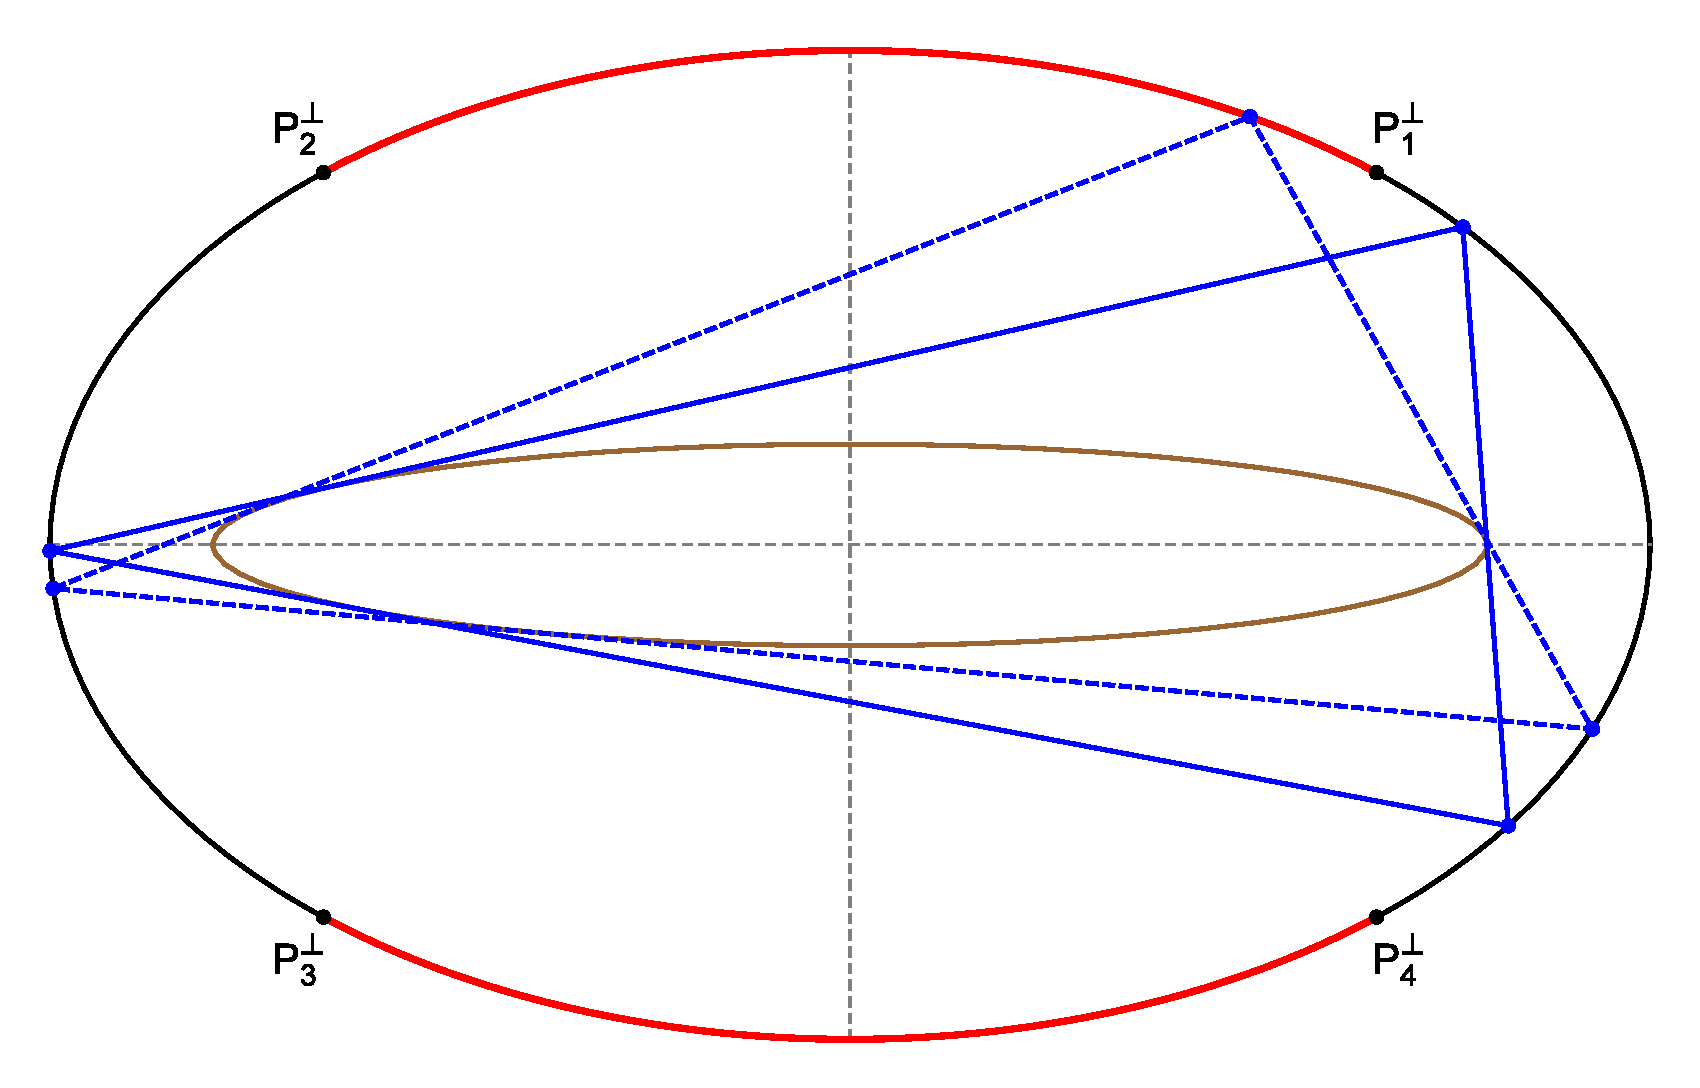
\includegraphics[width=.66\textwidth]{pics_eps_new/0080_rect_zones.eps}
    \caption{Two 3-periodics are shown: one acute (solid blue) and one obtuse (dashed blue) inscribed into an $a/b=1.618$ EB. Red arcs along the top and bottom halves of the EB indicate that when a 3-periodic vertex is there, the 3-periodic is obtuse. These only exist when $a/b>\alpha_4{\simeq}1.352$.}
    \label{fig:rect_zones}
\end{figure}

Consider the elliptic arc along the EB between $({\pm}x^\perp,y^\perp)$. When a vertex of the 3-periodic lies within  (resp. outside) this interval, the 3-periodic is obtuse (resp. acute).

\begin{proposition}
When $a/b>\alpha_4$, the locus of the center of the Orthic CB has four pieces: 2 for when the 3-periodic is acute (equal to the $X_6$ locus), and 2 when it is obtuse (equal to the locus of $X_6$ of $T''=P_2P_3X_4$.
\end{proposition}

\begin{proof}
It is well-known that \cite{etc} an acute triangle $T$ has an Orthic whose vertices lie on the sidelines. Furthermore the Orthic's Mittenpunkt coincides with the Symmedian $X_6$ of $T$. Also known is the fact that:

\begin{remark}
Let triangle $T'=P_1P_2P_3$ be obtuse on $P_1$. Its Orthic has one vertex on $P_2P_3$ and  two others exterior to $T'$. Its Orthocenter $X_4$ is also exterior. Furthermore, the Orthic's Mittenpunkt is the Symmedian Point $X_6$ of acute triangle $T''=P_2P_3X_4$.
\end{remark}

To see this, notice the Orthic of $T''$ is also\footnote{The anti-orthic pre-images of $T'$ are both the 3-periodic and $T''$.} $T'$. $T''$ must be acute since its Orthocenter is $P_2$.
\end{proof}

The CB of the orthic is shown in Figures~\ref{fig:cb_ort} for four 3-periodic configurations in an EB whose $a/b>\alpha_4$.

\begin{proposition}

The coordinates $({\pm}x^*,{\pm}y^*)$ where the locus of the center of the Orthic's CB transitions from one curve to the other are given by:

\begin{align*}
x^*=&\frac{x^{\perp}}{c^6}\left(a^6+2 a^2 b^4- b^2 \delta(3 a^2  +b^2)    +b^6\right)\\
%\frac{a^2 \sqrt{a^4+3 b^4-4 b^2 \delta } \left(a^6+2 a^2 b^4-3 a^2 b^2 \delta +b^6-b^4 \delta \right)}{c^9} \\
%=\frac{a^2 x^{\perp}}{a^2+b^2} \\
y^* =&-\frac{y^{\perp}}{c^6}\left(b^6+2 a^4 b^2 -  a^2 \delta (3 b^2 +a^2)   \delta+a^6\right)
   %\frac{b^2 \sqrt{-3 a^4+4
 %  a^2 \delta -b^4} \left(-a^6-2 a^4 b^2+a^4 \delta +3 a^2 b^2 \delta -b^6\right)}{c^9}\\
  % =\frac{b^2y^{\perp}}{a^2+b^2}
\end{align*}

\end{proposition}

\begin{proof}
Let $P_1=(x_1,y_1)$ be the right-triangle vertex of a 3-periodic, given by $(x^\perp,y^\perp)$ as in \eqref{eqn:xperp}. Using \cite{garcia2019-incenter}, obtain $P_2=(p_{2x}/q_2, p_{2y}/q_2)$ and $P_3=(p_{3x}/q_3, p_{3y}/q_3)$, with:
 
 \begin{align*}
     p_{2x}= &b^4 c^2 x_1^3 -2 a^4 b^2 x_1^2 y_1+a^4 c^2 x_1 y_1^2-2 a^6 y_1^3\\
     %
     p_{2y}=&2 b^6 x_1^3-b^4 c^2  x_1^2 y_1+2 a^2 b^4x_1 y_1^2-a^4 c^2 y_1^3\\
     q_2=&b^4 (a^2+b^2) x_1^2-2 a^2 b^2c^2 x_1 y_1 +a^4 (a^2+b^2) y_1^2\\
     p_{3x}=& b^4 c^2 x_1^3  +2 a^4 b^2 x_1^2 y_1+a^4 c^2 x_1 y_1^2+a^6 y_1^3\\
     p_{3y}=&-2 b^6 x_1^3 -b^4 c^2 x_1^2 y_1-2 a^2 b^4 x_1 y_1^2-a^4 c^2 y_1^3 \\
     q_3=&b^4 (a^2+b^2) x_1^2+2 a^2 b^2c^2 x_1 y_1+a^4 (a^2+b^2) y_1^2
 \end{align*}


It can be shown the Symmedian point $X_6$ of a right-triangle is the midpoint of its right-angle vertex altitude. Computing $X_6$ using this property leads to the result.
\end{proof}

    
Let $\alpha_{eq}=\sqrt{4 \sqrt{3}-3}\,{\simeq}\,1.982$ be the only positive root of $x^4 + 6 x^2 - 39$. It can be shown, see Figure~\ref{fig:cb_ort_equi}:

\begin{proposition}
At $a/b=\alpha_{eq}$, the locus of the Orthic CB is tangent to EB's top and bottom vertices. If a 3-periodic vertex is there, the Orthic is equilateral.
\end{proposition}

\begin{proof}
Let $T$ be an equilateral with side $s_{eq}$ and center $C$. Let $h$ be the distance from any vertex of $T$ to $C$. It can be easily shown that $h/s_{eq}=\sqrt{3}/3$. Let $T'$ be the Excentral Triangle of $T$: its sides are $2s_{eq}$. Now consider the upside down equilateral in Figure~\ref{fig:cb_ort_equi}, which is the Orthic of an upright isosceles 3-periodic. $h$ is clearly the 3-periodic's height and $2s_{eq}$ is its base. The height and width of the upright isosceles are obtained from explicit expressions for the vertices \cite{garcia2019-incenter}:

\begin{align*}
    s_{eq}=\frac{\alpha^2}{\alpha^2-1}\sqrt{2\delta-\alpha^2-1},\;\;\;h=\frac{\alpha^2+\delta+1}{\alpha^2+\delta}
\end{align*}

\noindent where $\alpha=a/b$. Setting $h/s_{eq}=\sqrt{3}/3$ and solving for $\alpha$ yields the required result for $\alpha_{eq}$.
\end{proof}

\begin{figure}
    \centering
    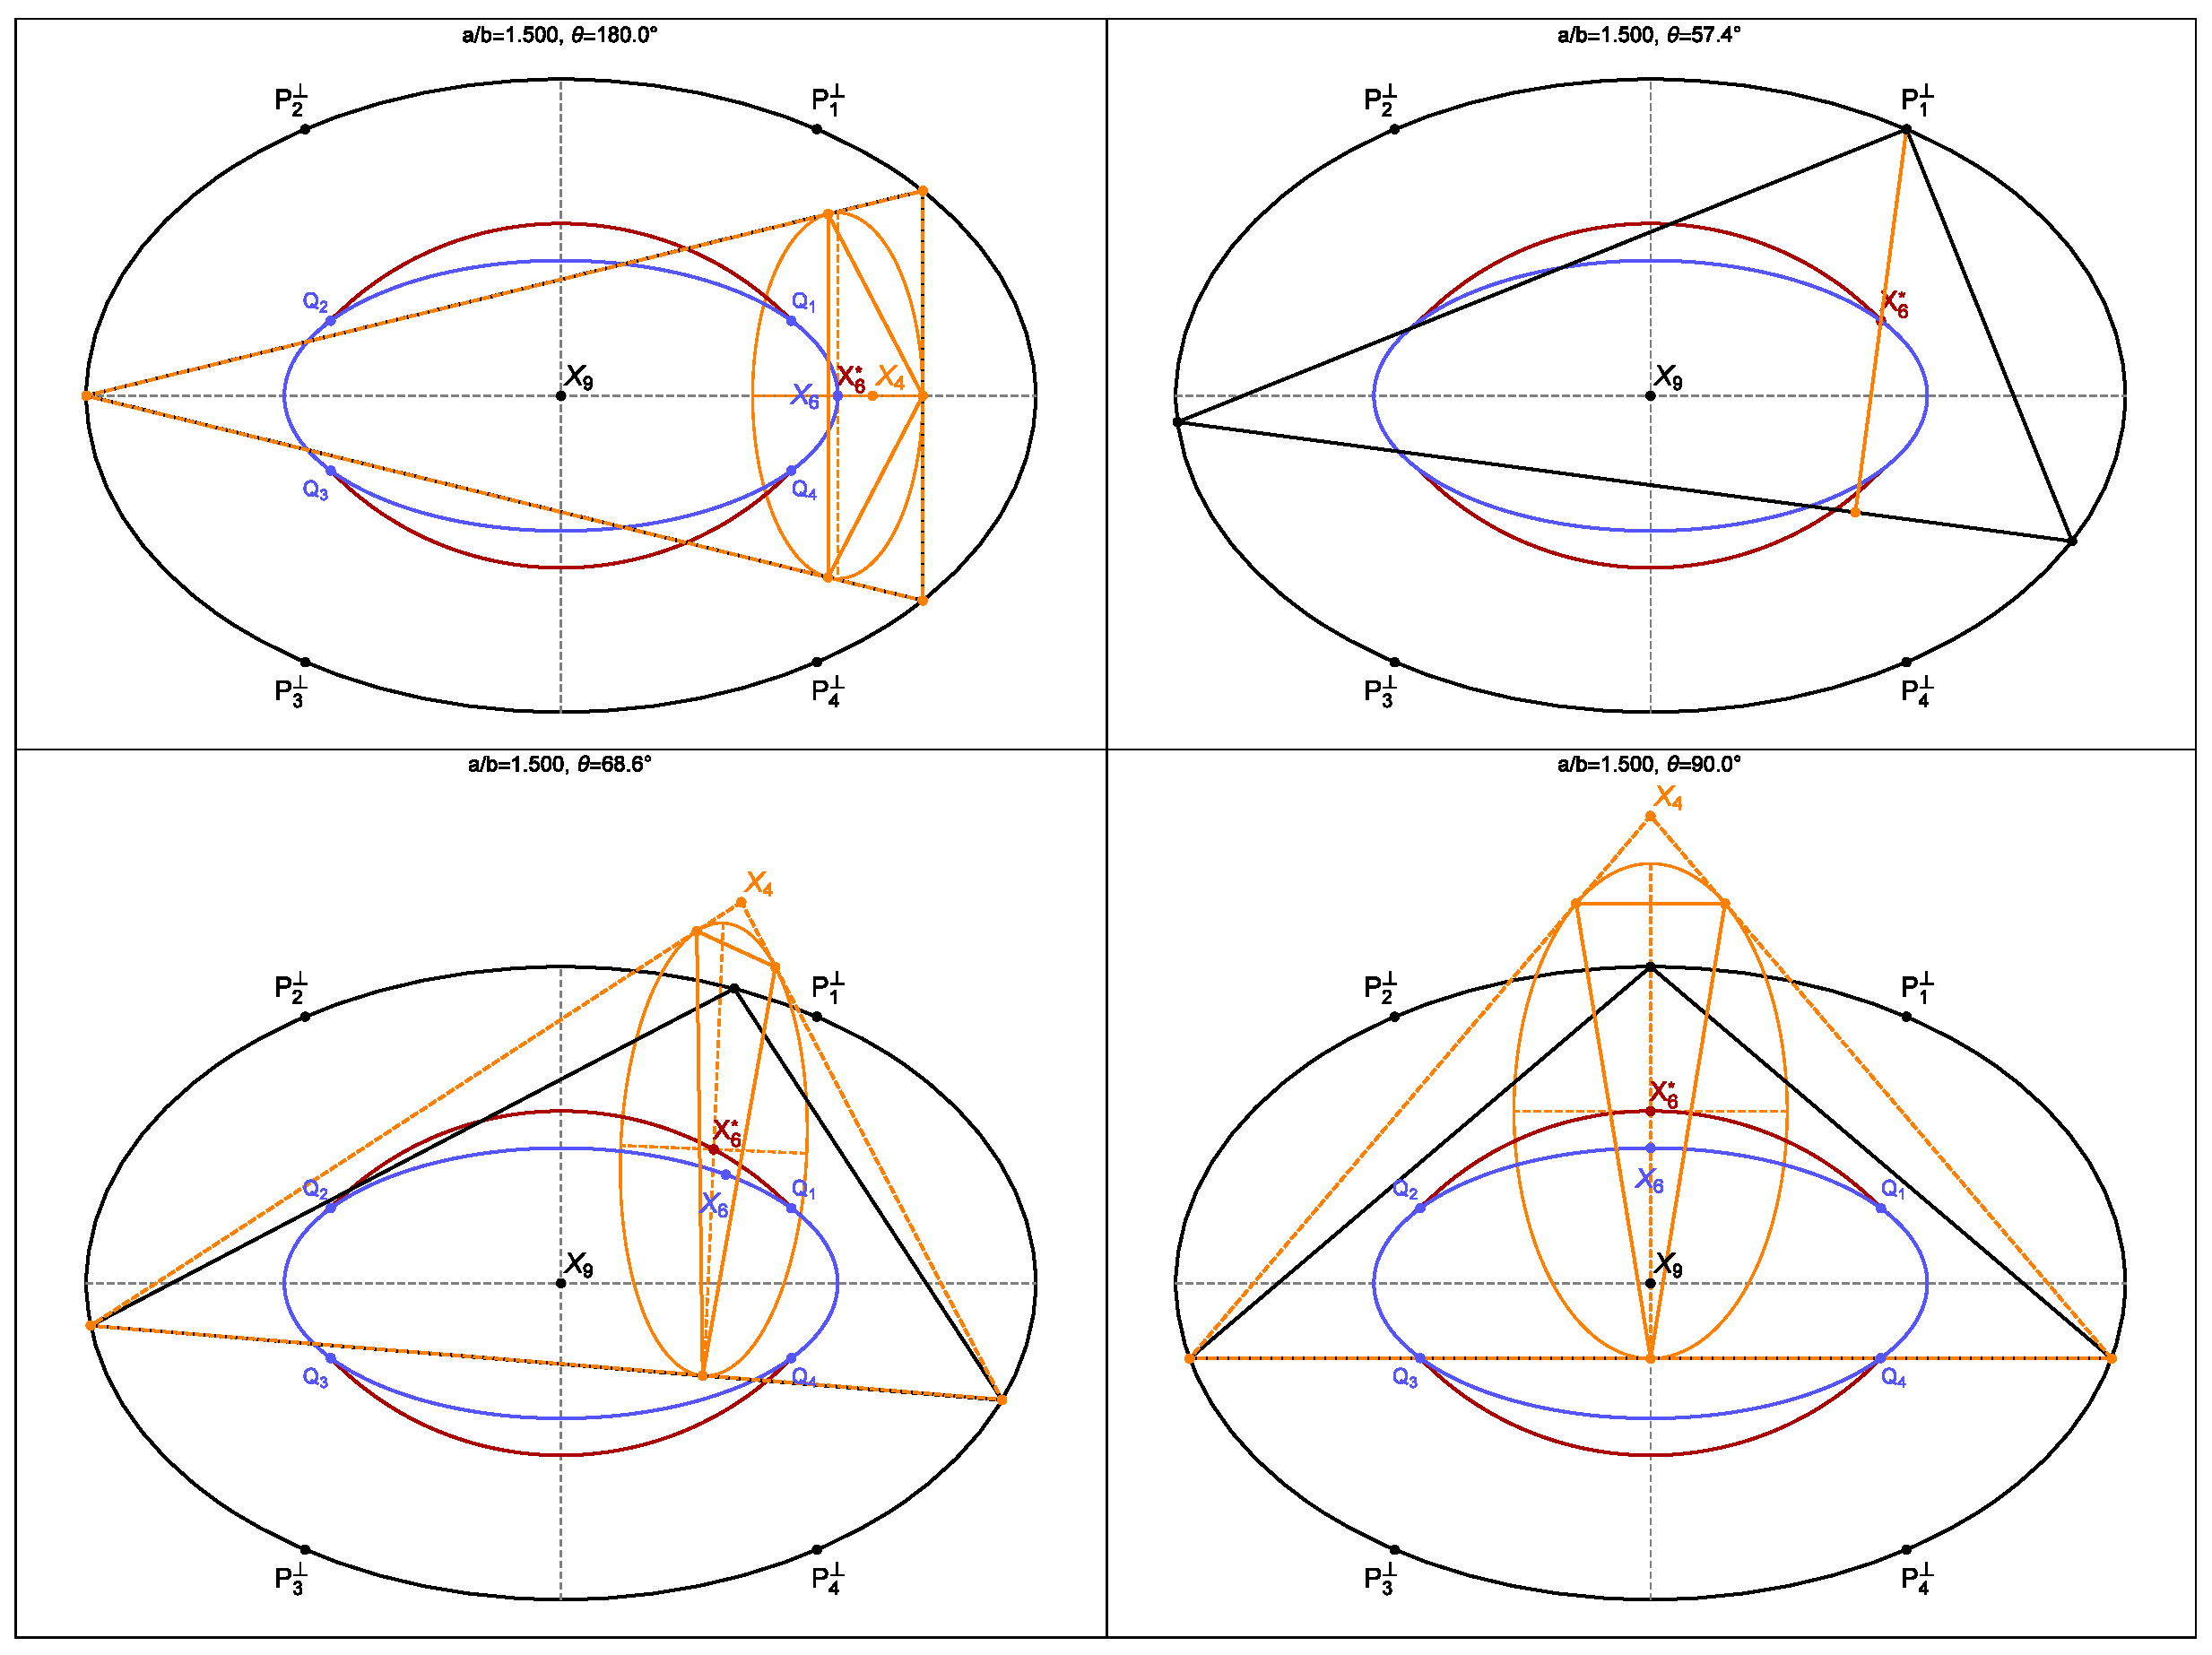
\includegraphics[width=\textwidth]{pics_eps_new/0030_cb_ort.eps}
    \caption{Orthic CB for an EB with $a/b=1.5>\alpha_4$, i.e., containing obtuse 3-periodics, which occur when a 3-periodic vertex lies on the top or bottom areas of the EB between the $P^\perp$. \textbf{Top left}: 3-periodic is sideways isosceles and acute (vertices outside $P^\perp$, so 3 orthic vertices lie on sidelines. The Orthic CB centers is simply the mittenpunkt of the Orthic, i.e, $X_6$ of the 3-periodic (blue curve: a convex quartic \cite{garcia2020-ellipses}). \textbf{Top right}: The position when a vertex is at a $P^\perp$ and the 3-periodic is a right triangle: its Orthic and CB degenerate to a segment. Here the CB center is at a first (of four) transition points shown in the other insets as $Q_i$, $i=1,2,3,4$. \textbf{Bottom left}: The 3-periodic is obtuse, the Orthic has two exterior vertices, and the center of the CB switches to the Symmedian of $T''=P_1P_2X_4$ (red portion of locus). \textbf{Bottom right:}. The 3-periodic is an upright isosceles, still obtuse, the center of the Orthic CB reaches its highest point along its locus (red). \textbf{Video}: \cite[PL\#06]{reznik2020-playlist-circum}.}
    \label{fig:cb_ort}
\end{figure}

\begin{figure}
    \centering
    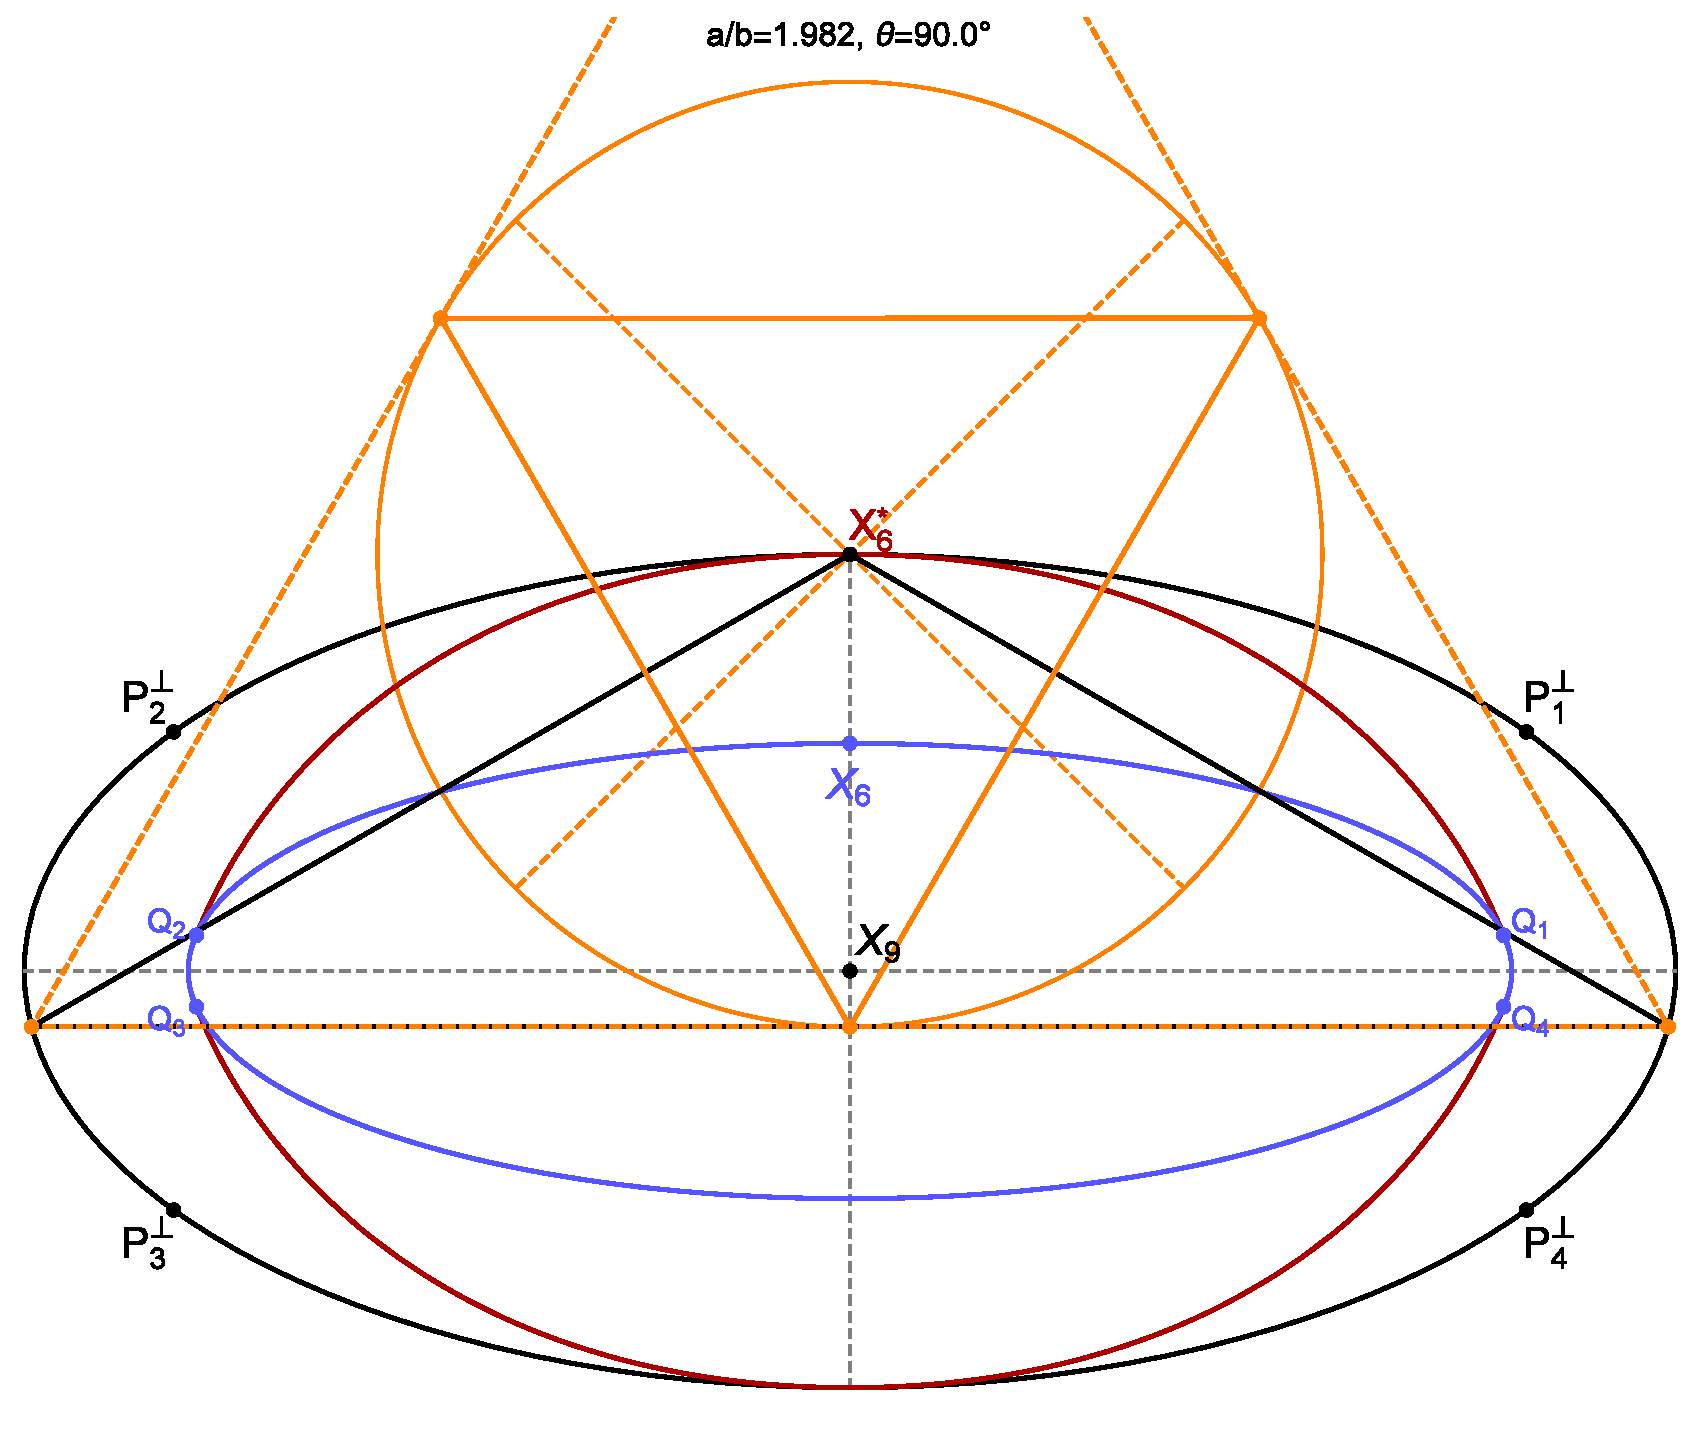
\includegraphics[width=\textwidth]{pics_eps_new/0040_cb_ort_equi.eps}
    \caption{At $a/b=\alpha_{eq}{\simeq}1.982$, the Orthic is an equilateral triangle when a 3-periodic vertex lies on a top or bottom vertex of the EB. Therefore its CB is a circle.}
    \label{fig:cb_ort_equi}
\end{figure}